\begin{figure}[h]
    \centering
    \begin{subfigure}[b]{0.24\textwidth}
        \centering
        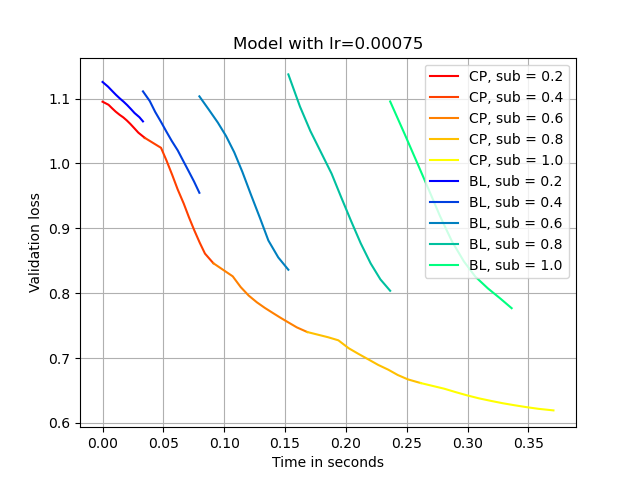
\includegraphics[width=\textwidth]{figures/22_07/iris/loss_time_0.00075.png}
        \caption{IRIS}
        \label{fig:13a}
    \end{subfigure}
    %\hfill
    \begin{subfigure}[b]{0.24\textwidth}
        \centering
        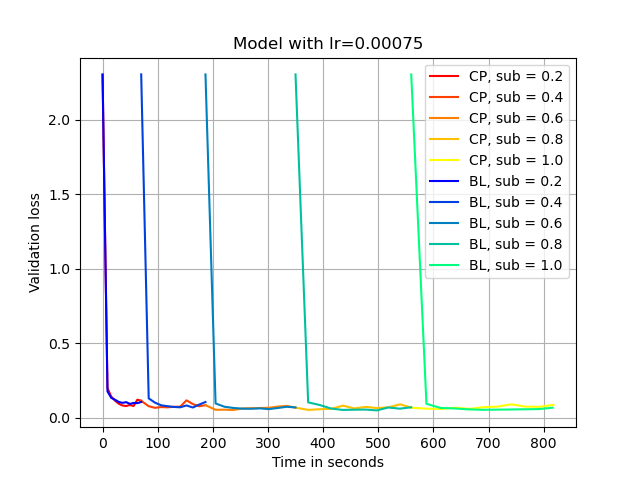
\includegraphics[width=\textwidth]{figures/22_07/10ep/loss_time_0.00075.png}
        \caption{MNIST 10 epochs}
        \label{fig:13b}
    \end{subfigure}
    %\hfill
    \begin{subfigure}[b]{0.24\textwidth}
        \centering
        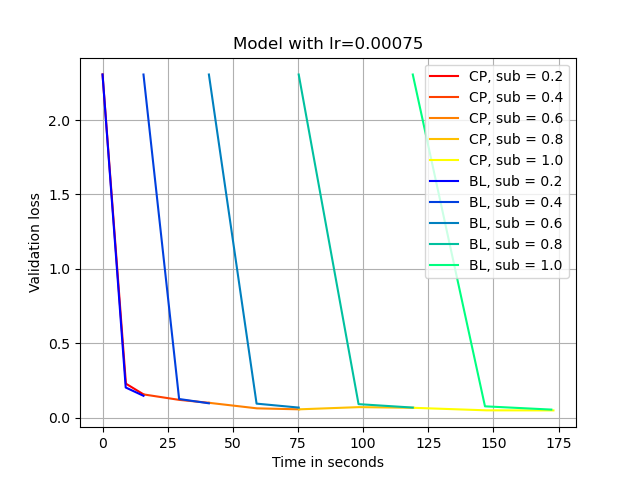
\includegraphics[width=\textwidth]{figures/22_07/2ep/loss_time_0.00075.png}
        \caption{MNIST 2 epochs}
        \label{fig:13c}
    \end{subfigure}
    %\hfill
    \begin{subfigure}[b]{0.24\textwidth}
        \centering
        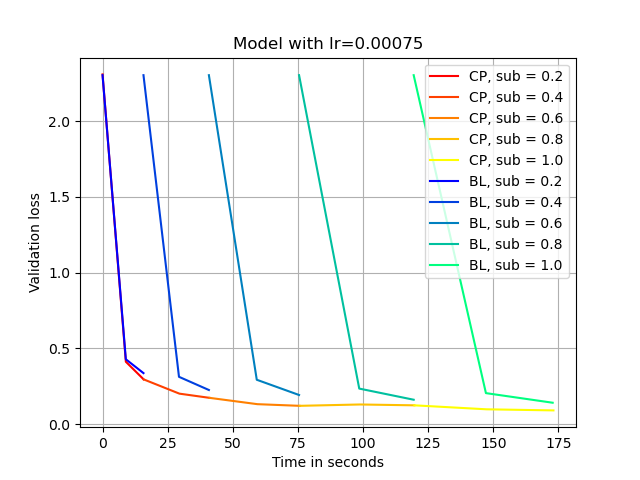
\includegraphics[width=\textwidth]{figures/22_07/2ep_smaller/loss_time_0.00075.png}
        \caption{MNIST 2 epochs, small model}
        \label{fig:13d}
    \end{subfigure}
    \caption{Visualization of validation loss versus training time for Adam optimizer and learning rate $7.5e^{-4}$}
    \label{fig:three graphs}
\end{figure}

\begin{figure}[h]
    \centering
    \begin{subfigure}[b]{0.24\textwidth}
        \centering
        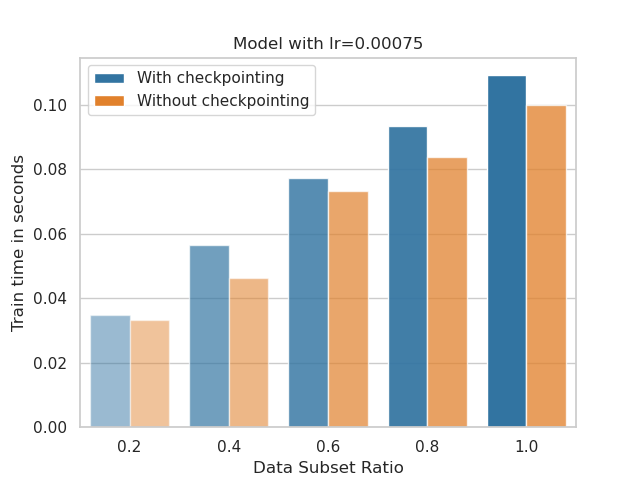
\includegraphics[width=\textwidth]{figures/22_07/iris/train_subset_0.00075.png}
        \caption{IRIS}
        \label{fig:19a}
    \end{subfigure}
    %\hfill
    \begin{subfigure}[b]{0.24\textwidth}
        \centering
        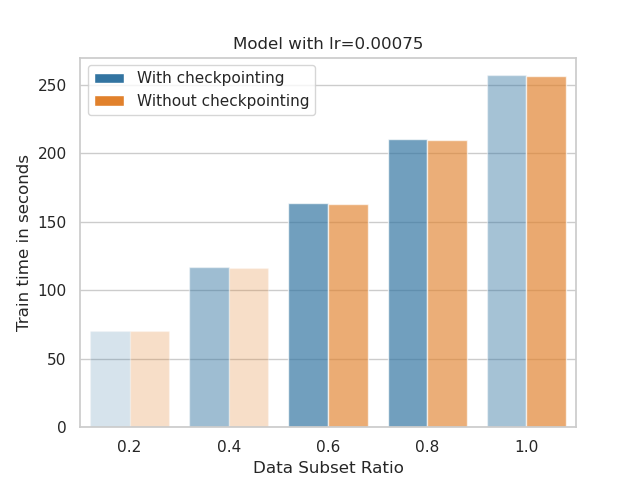
\includegraphics[width=\textwidth]{figures/22_07/10ep/train_subset_0.00075.png}
        \caption{MNIST 10 epochs}
        \label{fig:19b}
    \end{subfigure}
    %\hfill
    \begin{subfigure}[b]{0.24\textwidth}
        \centering
        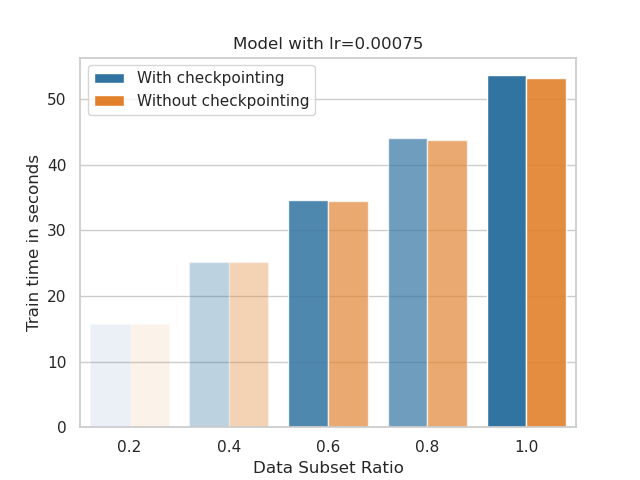
\includegraphics[width=\textwidth]{figures/22_07/2ep/train_subset_0.00075.png}
        \caption{MNIST 2 epochs}
        \label{fig:19c}
    \end{subfigure}
    %\hfill
    \begin{subfigure}[b]{0.24\textwidth}
        \centering
        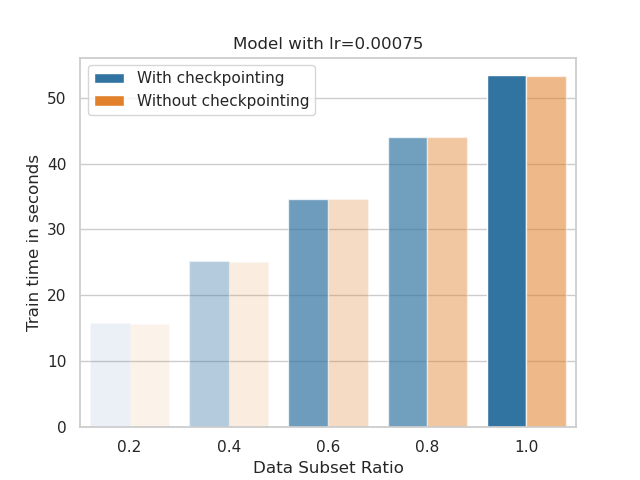
\includegraphics[width=\textwidth]{figures/22_07/2ep_smaller/train_subset_0.00075.png}
        \caption{MNIST 2 epochs, small model}
        \label{fig:19d}
    \end{subfigure}
    \caption{Visualization of the training time for every data subset ratio. A higher opacity means small validation performance difference to the optimum. An Adam optimizer and learning rate $7.5e^{-4}$ were used}
    \label{fig:19}
\end{figure}